\documentclass{standalone}
 
% Required package
\usepackage{tikz}
\usepackage{amssymb}
\usepackage{ntheorem}
\usepackage{tensor}
%\usepackage{physics}
\usepackage[italicdiff]{physics}
\usepackage{calc}
\usepackage{mathrsfs}
 \usetikzlibrary {backgrounds,mindmap}
 \usetikzlibrary{decorations.pathmorphing,decorations.markings}
\usetikzlibrary{decorations.pathreplacing} %
\begin{document}
 
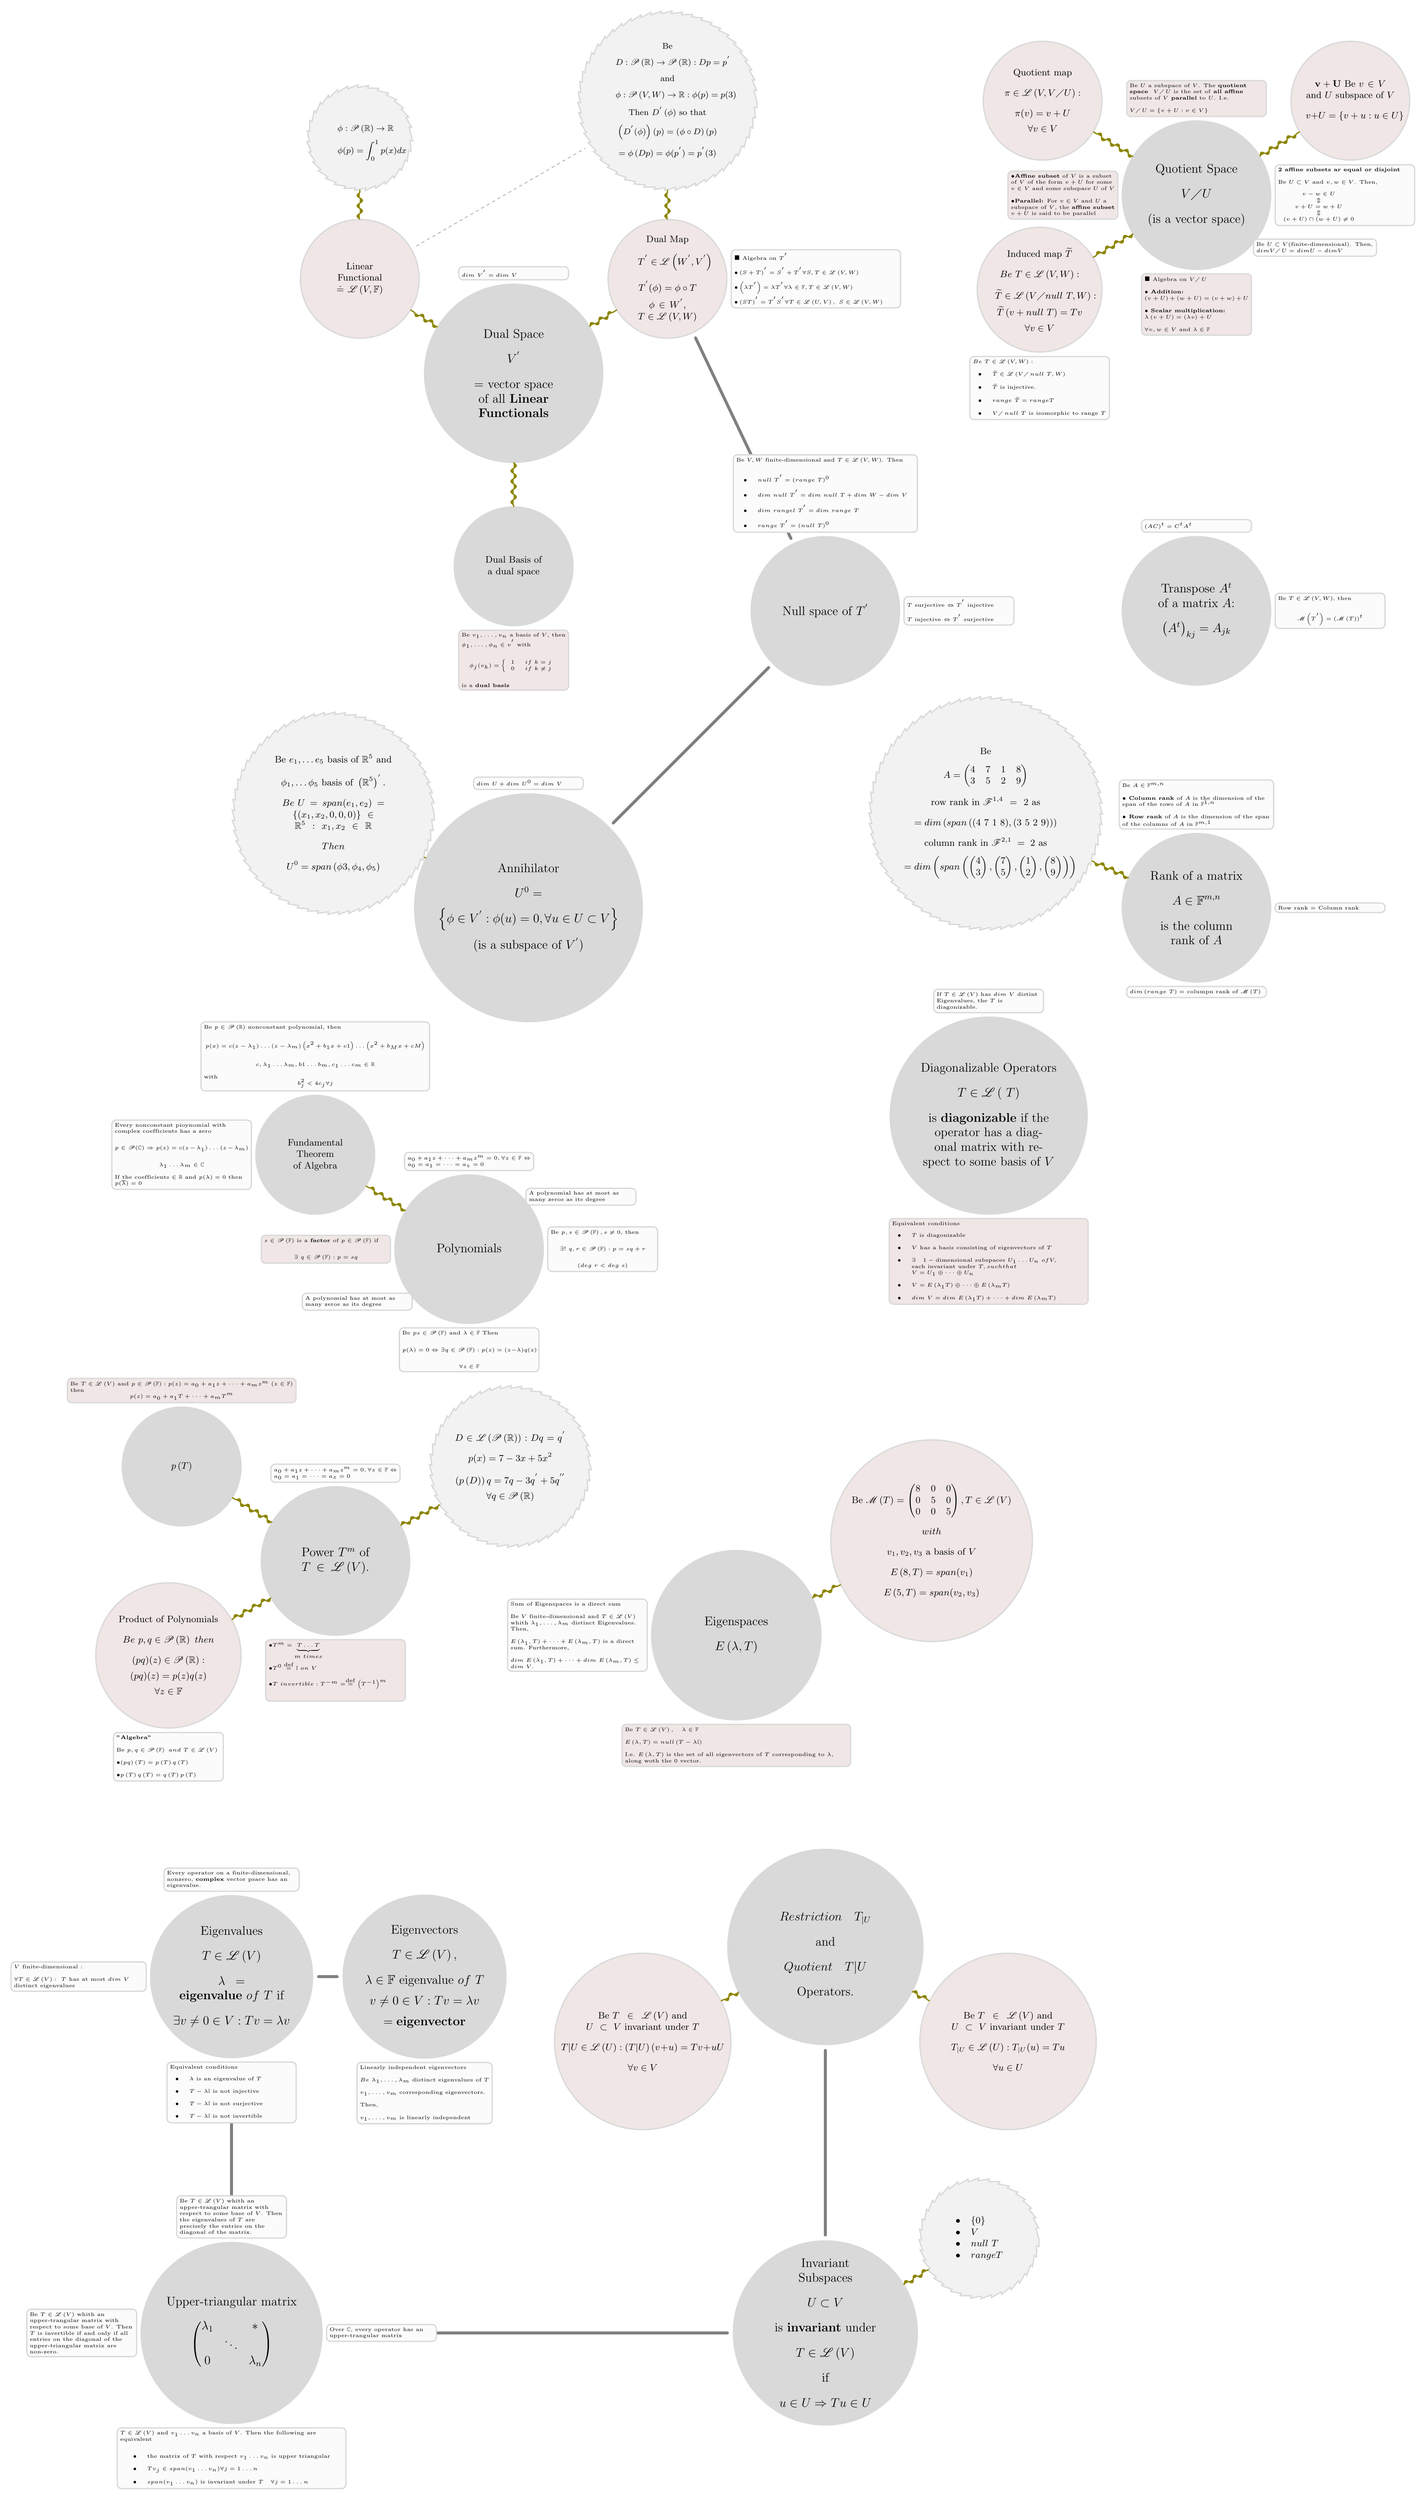
\begin{tikzpicture}[
    mindmap,
    concept color = gray!30,
    every node/.style = {concept},
    grow cyclic,
    minimum size=5cm,
    every annotation/.style={fill=gray!3},
    level 1/.append style = {
        concept color = gray!30,
        minimum size=4cm,
        level distance = 4.5cm,
        sibling angle = 120
    },
    level 2/.append style = {
        concept color = gray!30,
        minimum size=3.5cm,
        level distance = 3cm,
        sibling angle = 45
    },
    level 3/.append style = {
        concept color = gray!30,
        minimum size=3.5cm,
        level distance = 3cm,
        sibling angle = 45
    }
]
\tikzstyle{circle connection bar}=[to path={
  [every circle connection bar]
  decorate [decoration={snake}]
  { -- (\tikztotarget) \tikztonodes}
},
append after command={[fill=olive,draw=olive]}
]

\tikzstyle{example}=[{circle,decoration=saw,decorate,fill=gray!10,inner sep=8pt}]
\definecolor{def}{RGB}{240,230,230}
 
\coordinate(N1) at (-13.5,73) {} {} {} {} {} {} {} ;
\coordinate(N2) at (9.5,79) {} {} {} {} {};
\coordinate(N3) at (-13,55) {} {} {} {} {} {} ;
\coordinate(N4) at (-3,65) {} {} {} {} {} {} {} {};
\coordinate(N5) at (9.5,65) {} {} {};
\coordinate(N6) at (9.5,55) {} {} {} {};
\coordinate(N7) at (-15,43.5) {} {} {} {} {} {} ;
\coordinate(N8) at (-19.5,33) {} {} {} {} ;
\coordinate(N9) at (-3,7) {} {} {} {} ;
\coordinate(N10) at (-23,19) {} {} {} {} ;
\coordinate(N11) at (-16.5,19) {} {} {} {} {} {} {} {} {} {} ;
\coordinate(N12) at (-3,20) {} {} {} {} {} ;
\coordinate(N13) at (-23,7) {} {} {} {} {} ;
\coordinate(N14) at (-6,30.5) {} {} {} {} {} {};
\coordinate(N15) at (2.5,48) {} {} {} {} {} {} {};
\coordinate(N16) at (-37.5,42) {} {} {};
\coordinate(N17) at (-13,23.5) {} {} {} {} {} {} {};
\coordinate(N18) at (-33.5,74) {} {} {} {} {} {} {} {};
\coordinate(N19) at (-45,55.5) {};
\coordinate(N20) at (-1.5,50) {} {};




%%Dual Space
\node (VS) [concept,minimum size=6cm]
 at (N1){Dual Space $$V^{'}$$= vector space of all \textbf{Linear Functionals}  }
child [grow = south ] {node[below](VS3)   {Dual Basis of a dual space}}
child [grow = north east] {node[right,fill=def](VS4)   {Dual Map $$T^{'} \in \mathscr{L}\left(W^{'}, V^{'}\right) $$ $$ T^{'}(\phi)=\phi\circ T $$ $\phi \in W^{'},$ $ T \in  \mathscr{L}\left(V,W\right)$}
child [grow = north ] {node[text width = 3.5cm,above, example](VS41)   {Be $$D:\mathscr{P}\left(\mathbb{R}\right)\rightarrow \mathscr{P}\left(\mathbb{R}\right): Dp = p^{'}$$ and  $$\phi:  \mathscr{P}\left(V,W\right)\rightarrow \mathbb{R}: \phi(p)= p(3)$$ $\text{Then } D^{'}\left(\phi\right)$ so that $$ \left(D^{'}(\phi)\right)(p)= \left(\phi\circ D\right)(p) $$ $$= \phi\left(Dp\right) = \phi (p^{'}) = p^{'}(3)$$ }}}
child [grow = north west]{node[left,fill=def](VS1)  { Linear Functional $\doteq \mathscr{L}\left(V,\mathbb{F}\right)$}
child [grow = north ] {node[above,example](VS2)   {$$\phi: \mathscr{P}\left(\mathbb{R}\right)\rightarrow \mathbb{R}$$ $$ \phi(p) = \int_0^1 p(x)dx$$ }}
};
\node [annotation,above] at (VS.north){$dim\  V^{'} = dim \ V$  };
\node [annotation,below,fill = def] at (VS3.south){Be $v_1,\dots , v_n$ a basis of $V$, then $\phi_1,\dots,\phi_n \in v^{'}$    with $$\phi_j (v_k) = \left\{\begin{array}{ll} 1& if \ k=j\\ 0& if \ k\ne j\end{array}\right. $$ is a \textbf{dual basis} };
\node [annotation,right,text width = 5.5cm] at (VS4.east){{$\blacksquare$         Algebra on $T^{'}$\newline\newline
$\bullet \left(S+T\right)^{'}=  S^{'}+T^{'} \forall S,T \in \mathscr{L}\left(V,W\right)$\newline\newline
$\bullet\left (\lambda T^{'}\right)= \lambda T^{'} \forall \lambda \in \mathbb{F}, T \in \mathscr{L}\left(V,W\right)$\newline\newline 
$\bullet\left (S T\right)^{'}=T^{'} S^{'}\forall T \in\mathscr{L}\left(U,V\right),\   S \in \mathscr{L}\left(V,W\right)$} };




%%Quotient Space 
\node (QS) at (N2){Quotient Space  $$V\diagup U$$ (is a vector space)}
child  [grow = north east, text width = 3cm]{node[right,fill=def](QS1) {$\mathbf{v+U}$
Be $v\in V$ and $U \text{ subspace of } V$ $$v+U= \left\{ v+u: u\in U\right\}$$}}
child  [grow = north west, text width = 3cm]{node[left,fill=def](QS2) {Quotient map $$\pi \in \mathscr{L}\left(V,V\diagup U\right):$$ $$ \pi(v)= v+U$$  $$\forall v \in V$$}}
child   [grow = south west, text width = 3cm]{node [left,fill=def](QS3) {Induced map $\widetilde{T}$ $$Be \ T \in \mathscr{L}\left(V,W\right):$$ $$\widetilde{T} \in \mathscr{L}\left(V\diagup null \ T,W\right):$$ $$ \widetilde{T}\left(v+ null \ T\right) = Tv$$  $$\forall v \in V$$}}
;
\node [annotation,above ,fill = def,text width=4.5cm] at (QS.north){Be $U$ a subspace of $V$. The \textbf{quotient space } $V\diagup U$ is the set of \textbf{all affine } subsets of $V$ \textbf{parallel} to $U$. I.e.\newline\newline
$V\diagup U = \left\{ v+U: v\in V\right\}$};
\node [annotation,below,fill = def,] at (QS.south){$\blacksquare$         Algebra on $V\diagup U$\newline\newline
$\bullet$ \textbf{Addition: }$\left(v+U\right)+\left(w+U\right)= (v+w) +U$\newline\newline
$\bullet$ \textbf{Scalar multiplication: }$\lambda\left(v+U\right)= \left(\lambda v\right) +U$\newline\newline $\forall v,w \in V$ and $\lambda \in \mathbb{F}$};
\node [annotation,left,fill = def] at (QS.west){$\bullet$\textbf{Affine subset} of $V$ is a subset of $V$ of the form $v+U$ for some $v\in V$ and some subspace $U$ of $V$\newline\newline
$\bullet$\textbf{Parallel: }For $v\in V$ and $U$ a subspace of $V$, the \textbf{affine subset} $ v+U$ is said to be parallel};
\node [annotation,right,text width=4.5cm] at (QS.east){\textbf{2 affine subsets ar equal or disjoint}\newline \newline Be $ U \subset V$ and $v,w \in V$. Then, \newline
\newline $\begin{matrix}v-w\in U \\  \Updownarrow \\ v+U=w+U  \\ \Updownarrow \\\left(v+U\right) \cap\left( w+U\right) \ne 0 \end{matrix}$};
\node [annotation,right,,text width=3.95cm] at (QS.south east){ Be $ U \subset V$(finite-dimensional). Then,  $dim V\diagup U = dim U - dim V$};
\node [annotation,below,,text width=4.5cm] at (QS3.south){ $Be \ T \in \mathscr{L}\left(V,W\right):$\newline\newline $\begin{array}{ll}
\bullet&\widetilde{T} \in \mathscr{L}\left(V\diagup null \ T,W\right)\\ \\
\bullet&\widetilde{T} \text{ is injective.}\\ \\
\bullet& range \ \widetilde{T} = range  T\\ \\
\bullet&V\diagup null \ T \text{ is isomorphic to range } T
\end{array}$};




%%Annihilator
\node [text width =7cm](Anh) at (N3){Annihilator $$U^{0}= $$ $$\left\{\phi \in V^{'}: \phi(u)=0,  \forall u\in U \subset V\right\}$$(is a subspace of $V^{'}$)}
child  [grow = north west, text width = 4.5cm]{node[example,left](Anh1) {Be $e_1, \dots e_5$ basis of $\mathbb{R}^5$ and  $$\phi_1, \dots \phi_5 \text{ basis of }\left(\mathbb{R}^5\right)^{'}.$$ $Be \ U = span(e_1,e_2) = \left\{(x_1,x_2,0,0,0)\right\}\in \mathbb{R}^5:x_1,x_2 \in \mathbb{R}$ $$Then$$ $$ U^{0}= span\left(\phi3,\phi_4,\phi_5\right) $$ }}
;
\node [annotation,above ,] at (Anh.north){$dim \ U + dim \ U^{0} = dim \ V$};

%%Null space of T^'
\node [](NSTp) at (N4){Null space of $T^{'}$};
\node [annotation,above ,text width =6cm] at (NSTp.north){Be $V, W$ finite-dimensional and $T\in\mathscr{L}\left(V,W\right)$. Then
$$\begin{array}{ll}\bullet& null \ T^{'} = \left(range\ T\right)^{0}\\\\
\bullet & dim \ null \ T^{'}= dim \ null \ T+dim \ W-dim \  V\\\\
\bullet& dim \ rangel \ T^{'}= dim \ range \ T\\\\
\bullet& range \ T^{'} =  \left(null\ T\right)^{0}
\end{array}$$};
\node [annotation,right ] at (NSTp.east){$T$ surjective $\Leftrightarrow T^{'}$ injective
\newline\newline $T$ injective $\Leftrightarrow T^{'}$ surjective};

%%Transpose of a matrix'
\node [](TpM) at (N5){Transpose $A^{t}$ of a matrix $A$:  $$ \left(A^t\right)_{kj} = A_{jk}$$};
\node [annotation,above] at (TpM.north){$\left(AC\right)^t = C^t A^t$};
\node [annotation,right ] at (TpM.east){Be $T\in \mathscr{L}\left(V,W\right)$, then $$ \mathscr{M}\left(T^{'}\right) =  \left(\mathscr{M}\left(T\right)\right)^{t}$$};

%%Rank of a matrix'
\node [](RoM) at (N6){Rank of a matrix $$A\in \mathbb{F}^{m,n}$$ is the column rank of $A$}
child  [grow = north west, text width = 5.5cm]{node[example,left](RoM1) {Be $$A=\left( \begin{matrix} 4&7&1&8\\
3&5&2&9\end{matrix} \right)$$ row rank in $\mathscr{F}^{1,4}= 2$ as $$=dim\left(span\left((4 \ 7\ 1\ 8),(3\ 5\ 2\ 9)\right)\right)$$ 
column rank in $\mathscr{F}^{2,1}= 2$ as$$=dim\left(span\left(\left(\begin{matrix}4\\ 3\end{matrix}\right),\left(\begin{matrix}7\\ 5\end{matrix}\right),\left(\begin{matrix}1\\ 2\end{matrix}\right),\left(\begin{matrix}8\\ 9\end{matrix}\right)\right)\right)$$}}
;
\node [annotation,above, text width= 5cm] at (RoM.north){Be $A \in \mathbb{F}^{m,n}$ \newline\newline 
$\bullet $\textbf{ Column rank} of $A$ is the dimension of the span of the rows of $A$ in $\mathbb{F}^{1,n}$
\newline\newline 
$\bullet $\textbf{ Row rank} of $A$ is the dimension of the span of the columns of $A$ in $\mathbb{F}^{m,1}$};
\node [annotation,right ] at (RoM.east){Row rank $=$ Column rank};
\node [annotation,below,text width= 4.5cm] at (RoM.south){$dim\left(range \ T \right)=$ columpn rank of $\mathscr{M}\left(T\right)$};

%%Polynomials
\node [](Poly) at (N7){Polynomials  }
child  [grow = north west, ]{node[left](Poly1) {Fundamental Theorem of Algebra}}
;
\node [annotation,above,text width = 4.15cm] at (Poly.north){$a_0+a_1z+\dots +a_mz^m=0, \forall z\in \mathbb{F}\Leftrightarrow a_0=a_1=\dots = a_z=0$};
\node [annotation,right ] at (Poly.east){Be $p,s \in \mathscr{P}\left(\mathbb{F}\right), s\ne 0$, then $$ \exists ! \ q,r \in \mathscr{P}\left(\mathbb{F}\right): p=sq+r$$  $$ (deg\ r < deg \ s)$$};
\node [annotation,left,text width = 4.15cm, fill=def] at (Poly.west){$s \in \mathscr{P}\left(\mathbb{F}\right)$ is a \textbf{factor} of $p \in \mathscr{P}\left(\mathbb{F}\right)$ if$$ \exists  \ q \in \mathscr{P}\left(\mathbb{F}\right): p=sq$$  };
\node [annotation,below,text width = 4.5cm] at (Poly.south){Be $ps \in \mathscr{P}\left(\mathbb{F}\right)$ and $\lambda \in \mathbb{F}$ Then $$p(\lambda)=0 \Leftrightarrow \exists q \in \mathscr{P}\left(\mathbb{F}\right): p(z)= (z-\lambda)q(z)$$  $$ \forall z\in \mathbb{F}$$ };
\node [annotation,left,text width = 3.5cm] at (Poly.south west){ A polynomial has at most as many zeros as its degree};
\node [annotation,right,text width = 3.5cm] at (Poly.north east){ A polynomial has at most as many zeros as its degree};
\node [annotation,left,text width = 4.5cm] at (Poly1.west){Every nonconstant pioynomial with complex coefficients has a  zero$$p\in \mathscr{P}(\mathbb{C})\Rightarrow p(z) = c(z-\lambda_1)\dots (z-\lambda_m)$$ $$ \lambda_1\dots \lambda_m\in \mathbb{C}$$
If the coefficients $\in \mathbb{R}$ and $ p(\lambda)=0$ then $ p(\overline{\lambda})=0$};
\node [annotation,above,text width = 7.5cm] at (Poly1.north){Be $ p\in \mathscr{P}\left(\mathbb{R}\right)$ nonconstant polynomial, then $$p(x) =c(z-\lambda_1)\dots (z-\lambda_m)\left(x^2+b_1x+c1\right)\dots\left(x^2+b_Mx+cM\right) $$ $$ c, \lambda_1\dots \lambda_m, b1\dots b_m, c_1\dots c_m  \in \mathbb{R}$$ with
$$ b_j^2 < 4c_j \forall j$$
};

%%Powers of T
\node [](PoT) at (N8){Power $T^m$ of $T\in\mathscr{L}\left(V\right)$.}
child  [grow = north west, ]{node[left](PoT1) {$p\left(T\right)$}}
child  [grow = north east, ]{node[right,example,text width = 4.cm](PoT2) {$D\in \mathscr{L}\left(\mathscr{P}\left(\mathbb{R}\right)\right): Dq=q^{'}$ $$p(x)=7-3x+5x^2$$ $$ \left(p\left(D\right)\right)q= 7q-3q^{'}+5q^{''}$$ $$\forall q\in \mathscr{P}\left(\mathbb{R}\right)$$}}
child  [grow = south west, ]{node[left,text width = 4.cm,fill=def](PoT3) {Product of Polynomials$$Be \ p,q \in \mathscr{P}\left(\mathbb{R}\right) \ then$$ $$(pq)(z)\in \mathscr{P}\left(\mathbb{R}\right): $$ $$(pq)(z)=p(z)q(z)$$  $$\forall z\in \mathbb{F}$$}}
;
\node [annotation,above,text width = 4.15cm] at (PoT.north){$a_0+a_1z+\dots +a_mz^m=0, \forall z\in \mathbb{F}\Leftrightarrow a_0=a_1=\dots = a_z=0$};
\node [annotation,below ] at (PoT3.south){\textbf{"Algebra"}\newline\newline Be $p,q\in  \mathscr{P}\left(\mathbb{F}\right) \ and \ T \in \mathscr{L}\left(V\right) $\newline\newline
$\bullet (pq)\left(T\right)= p\left(T\right) q\left(T\right)$ \newline\newline $ \bullet p\left(T\right) q\left(T\right)=q\left(T\right) p\left(T\right)$};
\node [annotation,below,text width = 4.5cm,fill=def] at (PoT.south){$\bullet T^m= \underbrace{T\dots T}_{m\ times}$\newline\newline
$\bullet T^0 \overset{\underset{\mathrm{def}}{}}{=} \mathbb{I} \ on \ V$\newline\newline
$\bullet T\ invertible: T^{-m} = \overset{\underset{\mathrm{def}}{}}{=} \left(T^{-1}\right)^m$\newline\newline};
\node [annotation,above,text width = 7.5cm, fill= def] at (PoT1.north){Be $T\in\mathscr{L}\left(V\right)$ and $p\in \mathscr{P}\left(\mathbb{F}\right): p(z)= a_0+a_1z+\dots +a_mz^m$  $(z\in \mathbb{F})$ then $$p(z)= a_0+a_1T+\dots +a_mT^m$$ 
};

%%Invariant Subspaces
\node [](InvS) at (N9){Invariant Subspaces $$U\subset V $$ is \textbf{invariant} under $$T\in\mathscr{L}\left(V\right)$$ if $$ u\in U\Rightarrow Tu\in U$$ }
child  [grow = north east, ]{node[right,example](InvS2) {$ \begin{array}{ll} \bullet & \{0\}\\
\bullet&V\\
\bullet& null \ T\\
\bullet& range T
\end{array}$}}
;

%%Eigenvalues
\node [text width = 4.15cm](Eigenval) at (N10){Eigenvalues $$T\in\mathscr{L}\left(V\right)$$ $\lambda=   \textbf{eigenvalue} \ of \ T  $ if $$ \exists v\neq 0 \in V:Tv=\lambda v$$ }
;
\node [annotation,below,text width = 4.15cm] at (Eigenval.south){Equivalent conditions\newline\newline $ \begin{array}{ll} 
\bullet & \lambda \text{ is an eigenvalue of } T\\\\
\bullet& T- \lambda \mathbb{I} \text{ is not injective }\\\\
\bullet&  T- \lambda \mathbb{I} \text{ is not surjective }\\\\
\bullet&  T- \lambda \mathbb{I} \text{ is not invertible }
\end{array}$};
\node [annotation,left,text width = 4.35cm] at (Eigenval.west){$V$ finite-dimensional :\newline\newline 
$\forall T\in \mathscr{L}\left(V\right): \ T $ has at most $dim \ V$ distinct eigenvalues};
\node [annotation,above,text width = 4.35cm] at (Eigenval.north){Every operator on a finite-dimensional, nonzero, \textbf{complex} vector psace has an eigenvalue.};


%%Eigenvectors
\node [text width = 4.15cm](Eigenvec) at (N11){Eigenvectors $$T\in\mathscr{L}\left(V\right),$$ $$\lambda\in \mathbb{F}  \text{ eigenvalue} \ of \ T  $$  $$v\neq 0 \in V:Tv=\lambda v$$ $$= \textbf{eigenvector} $$  }
;
\node [annotation,below,text width = 4.35cm] at (Eigenvec.south){Linearly independent eigenvectors \newline\newline $ Be \ \lambda_1,\dots , \lambda_m$ distinct eigenvalues of $T$\newline\newline $ v_1,\dots , v_m $ corresponding eigenvectors. \newline\newline Then,
\newline\newline $ v_1,\dots , v_m$ is linearly independent };

%%Restriction and Quotient Operators
\node [text width = 5.5cm](RQo) at (N12){$$Restriction \quad T_{|U}$$ and $$Quotient \quad T|U$$ Operators.}
child  [grow = south east, ]{node[right,text width = 5.5cm,fill=def] (RQo1){Be $T \in \mathscr{L}\left(V\right)$ and $U\subset V$ invariant under $T$ $$T_{|U} \in\mathscr{L}\left(U\right): T_{|U}(u)=Tu $$ $$\forall u \in U$$ }}
child  [grow = south west, ]{node[left,text width = 5.5cm,fill=def](RQo2){Be $T \in \mathscr{L}\left(V\right)$ and $U\subset V$ invariant under $T$ $$T|U \in\mathscr{L}\left(U\right): \left(T|U\right)(v+u)=Tv+uU $$ $$\forall v \in V$$ }}
;


%%Upper-triangular matrix
\node [text width = 5.5cm](UTM) at (N13){Upper-triangular matrix$$\left(\begin{matrix} \lambda_1 & & *\\
&\ddots&\\
0& & \lambda_n
\end{matrix}\right)$$}
%child  [grow = south east, ]{node[right,text width = 5.5cm,fill=def] (UTM1){Be $T \in \mathscr{L}\left(V\right)$ and $U\subset V$ invariant under $T$ $$T_{|U} \in\mathscr{L}\left(U\right): T_{|U}(u)=Tu $$ $$\forall u \in U$$ }}
%child  [grow = south west, ]{node[left,text width = 5.5cm,fill=def](UTM2){Be $T \in \mathscr{L}\left(V\right)$ and $U\subset V$ invariant under $T$ $$T|U \in\mathscr{L}\left(U\right): \left(T|U\right)(v+u)=Tv+uU $$ $$\forall v \in V$$ }}
;
\node [annotation,below,text width = 7.5cm] at (UTM.south){$T\in\mathscr{L}\left(V\right)$ and $ v_1\dots v_n$ a basis of $V$. Then the following are equivalent
$$\begin{array}{ll}
\bullet & \text{the matrix of } T \text{ with respect  } v_1\dots v_n \text{ is upper triangular}\\\\
\bullet& Tv_j \in span (v_1\dots v_n) \forall j=1 \dots n\\\\
\bullet& span (v_1\dots v_n)\text{ is invariant under } T\quad  \forall j=1\dots n
\end{array}  $$};
\node [annotation,right,text width = 3.5cm] at (UTM.east){Over $\mathbb{C}$, every operator has an upper-trangular matrix};
\node [annotation,left,text width = 3.5cm] at (UTM.west){Be  $T \in \mathscr{L}\left(V\right) $ whith  an upper-trangular matrix with respect to some base of $V$. Then $T$ is invertible if and only if all entries on the diagonal of the upper-triangular matrix are non-zero.};
\node [annotation,above,text width = 3.5cm] at (UTM.north){Be  $T \in \mathscr{L}\left(V\right) $ whith an upper-trangular matrix with respect to some base of $V$. Then the eigenvalues of $T$ are precisely the entries on the diagonal of the matrix.};


%%Eigenspaces
\node [text width = 5.5cm](ES) at (N14){Eigenspaces $$E\left(\lambda, T\right)$$}
child  [grow = north east, ]{node[right,text width = 5.5cm,fill=def] (ES1){Be $\mathscr{M}\left(T\right)=\left(\begin{matrix}8&0&0\\ 0&5&0\\ 0&0&5\end{matrix}\right), T  \in \mathscr{L}\left(V\right)$ $$with$$ $v_1,v_2,v_3$ a basis of $V$
$$ E\left(8,T\right)= span(v_1) $$ $$E\left(5,T\right)= span(v_2,v_3)$$ }}
%child  [grow = south west, ]{node[left,text width = 5.5cm,fill=def](ES2){Be $T \in \mathscr{L}\left(V\right)$ and $U\subset V$ invariant under $T$ $$T|U \in\mathscr{L}\left(U\right): \left(T|U\right)(v+u)=Tv+uU $$ $$\forall v \in V$$ }}
;
\node [annotation,below,fill=def,text width = 7.5cm] at (ES.south){Be $T\in\mathscr{L}\left(V\right), \quad \lambda \in \mathbb{F}$ \newline\newline$E\left(\lambda, T\right)= null\left(T-\lambda\mathbb{I}\right)$\newline\newline I.e. $E\left(\lambda, T\right)$ is the set of all eigenvectors of $T$ corresponding to $\lambda$, along woth the $0$ vector. };
%\node [annotation,right,text width = 3.5cm] at (ES.east){Over $\mathbb{C}$, every operator has an upper-trangular matrix};
\node [annotation,left,text width = 4.5cm] at (ES.west){Sum of Eigenspaces is a direct sum\newline\newline Be  $V$ finite-dimensional and $T \in \mathscr{L}\left(V\right) $ whith  $\lambda_1, \dots,\lambda_m$ distinct Eigenvalues. Then, \newline\newline $E\left(\lambda_1,T\right)+\dots +E\left(\lambda_m,T\right)$ is a direct sum. Furthermore, \newline\newline  $dim\ E\left(\lambda_1,T\right)+\dots +dim\ E\left(\lambda_m,T\right)\le dim\ V$. };

%%Diagonalizable Operators
\node [text width = 5.5cm](DO) at (N15){Diagonalizable Operators $$T\in \mathscr{L}\left(\ T\right)$$ is \textbf{diagonizable} if the operator has a diagonal matrix with respect to some basis of $V$}
;
\node [annotation,below,fill=def,text width = 6.5cm] at (DO.south){ Equivalent conditions \newline\newline $\begin{array}{ll}\bullet&T \text{ is diagonizable}\\\\
\bullet&V \text{ has a basis consisting of eigenvectors of } T\\\\ 
\bullet&\exists \quad 1-\text{dimensional subspaces } U_1\dots U_n \ of V,\\
&\text{each invariant under }T, such that\\
&V= U_1\oplus\dots \oplus U_n\\\\
\bullet& V= E\left(\lambda_1 T \right)\oplus\dots \oplus E\left(\lambda_m T \right)\\\\
\bullet&dim\ V = dim\ E\left(\lambda_1 T \right) + \dots + dim\ E\left(\lambda_m T \right)
\end{array}$ };
\node [annotation,above] at (DO.north){ If $T\in \mathscr{L}\left(V\right)$ has $dim\ V$ distint Eigenvalues, the $T$ is diagonizable.};

\begin{pgfonlayer}{background}
\draw [concept connection, dashed,thin ]  (VS1) edge (VS41);
\draw [concept connection,  ]  (Anh) edge (NSTp);
\draw [concept connection,  ]  (VS4) edge (NSTp);
\draw [concept connection,  ]  (Eigenval) edge (Eigenvec);
\draw [concept connection,  ]  (Eigenval) edge (UTM);
\draw [concept connection,  ]  (InvS) edge (RQo);
\draw [concept connection,  ]  (InvS) edge (UTM);
  \end{pgfonlayer}
\end{tikzpicture}
 
\end{document}